% The entire content of this work (including the source code
% for TeX files and the generated PDF documents) by 
% Hongxiang Chen (nicknamed we.taper, or just Taper) is
% licensed under a 
% Creative Commons Attribution-NonCommercial-ShareAlike 4.0 
% International License (Link to the complete license text:
% http://creativecommons.org/licenses/by-nc-sa/4.0/).
\documentclass{article}

% My own physics package
% The following line load the package xparse with additional option to
% prevent the annoying warnings, which are caused by the package
% "physics" loaded in package "physicist-taper".
\usepackage[log-declarations=false]{xparse}
\usepackage{physicist-taper}
\makenomenclature % For an index of symbols.

\title{TR Invariant T.I.}
\date{\today}
\author{Taper}


\begin{document}


\maketitle
\abstract{
    An incomplete note of dissertation by Taylor Hughes
    \cite{Hughes2009}.
}
\tableofcontents
Start with chapter 2.

\section{Spectrum of \texorpdfstring{$(2+1)$}-d Lattice Dirac Model}
\label{sec:2+1d-LDirac Model}
\begin{align}
    H_{LD} &= \sum_{m,n}\left\{
        i \left[ c^\dagger_{m+1,n}\sigma^x c_{m,n}
            - c^\dagger_{m,n}\sigma^x c_{m+1,n}\right]
        + i \left[ c^\dagger_{m,n+1}\sigma^y c_{m,n}
            - c^\dagger_{m,n}\sigma^y c_{m,n+1} \right]
        \right.
        \nonumber\\
        &- \left[
            c^\dagger_{m+1,n}\sigma^z c_{m,n}
            + c^\dagger_{m,n}\sigma^z c_{m+1,n}
            + c^\dagger_{m,n+1}\sigma^z c_{m,n}
            + c^\dagger_{m,n}\sigma^z c_{m,n+1}
        \right]
        \nonumber\\
        & \left. + (2-m) c^\dagger_{m,n}\sigma^z c_{m,n}
        \vphantom{xx}\frac\hbar2
    \right\}
\end{align}

Above is the lattice model (eq.2.19) of \cite{Hughes2009}. Here it
should be noted that $c_{m,n}=(c_{u,m,n}, c_{v,m,n})$ for two degrees
of freedom. 

\subsection{Numerical Solution in Infinity Cylinder Geometry}
\label{sec:Numerical Solution in Infinity Cylinder Geometry}

This Hamiltonian is solved here with a infinite cylinder geometry, i.e.
the lattice is infinite in $x$ direction while being periodic in $y$
direction. Because of this special setup, the $p_x$ is still a good
quantum number. Therefore we can do a fourier expansion in $x$
direction:

\begin{equation}
    c_{m,n} = \frac{1}{\sqrt{L_x}} \sum_{p_x} e^{ip_x m} c_{p_x,n}
\end{equation}

The resulted Hamiltonian is 

\begin{align}
    \tilde H_{LD} = \sum_{n,p_x}\quad &
    2\sin(p_x) c^\dagger_{p_x,n}\sigma^x c_{p_x,n}
    +i \left[ c^\dagger_{p_x,n+1}\sigma^y c_{p_x,n} - 
        c^\dagger_{p_x,n+1}\sigma^y c_{p_x,n}\right]
    \nonumber\\
    &- \left[ 2\cos(p_x) c^\dagger_{p_x,n}\sigma^z c_{p_x,n}
        c^\dagger_{p_x,n+1}\sigma^z c_{p_x,n}
        + c^\dagger_{p_x,n}\sigma^z c_{p_x,n+1}
    \right]
    \nonumber\\
    &+ (2-m) c^\dagger_{p_x,n}\sigma^z c_{p_x,n}
\end{align}

This Hamiltonian can be solved by acting it on the test wavefunction:
\begin{equation}
    \ket{\psi_{p_x}} = \sum_n \psi_{p_x,n,u} c^\dagger_{p_x,n,u} +
                        \psi_{p_x,n,v} c^\dagger_{p_x,n,v} \ket{0}
\end{equation}

Note, in choosing the test wavefunction, $u$ and $v$ could not be
separated, because there is still interaction between the two
component in terms like $c^\dagger_{p_x,n}\sigma^x c_{p_x,n}$.
If we calculate $\tilde H_{LD}\ket{\psi_{p_x}} = E_{p_x}
\ket{\psi_{p_x}}$, we would get after careful calculation:

\begin{align}
    & \sum_n
    c^\dagger_{p_x,n} A   \psi_{p_x,n-1}
    + c^\dagger_{p_x,n} B \psi_{p_x,n} 
    + c^\dagger_{p_x,n} C \psi_{p_x,n+1}
    \nonumber\\
    &= E_{p_x} \sum_n c^\dagger_{p_x,n}\psi_{p_x,n}
\end{align}
where
\begin{align}
    c^\dagger_{p_x,n} &= \begin{pmatrix}
        c^\dagger_{p_x,n,u},  c^\dagger_{p_x,n,v}
    \end{pmatrix} \\
    A &= i\sigma^y - \sigma^z \\
    B &= 2\sin(p_x)\sigma^x - 2\cos(p_x)\sigma^z + (2-m)\sigma^z \\
    C &= -i\sigma^y - \sigma^z \\
    \psi_{p_x,n} &= \begin{pmatrix}
        \psi_{p_x,n,u} \\ \psi_{p_x,n,v}
    \end{pmatrix}
\end{align}

Suppose there is $N$ lattice in the $y$ direction. Then the periodic
boundary condition implies that $\psi_{N+1}=\psi_{n=1}$, and
$\psi_{n=0} = \psi_N$.

Therefore, the eigenvalue equation could be turned into a matrix form:
\begin{align}
    \label{eq:disc-eigeneq}
    H_{\text{disc}} \psi \equiv 
    \begin{pmatrix}
        B   & C &        &   & A \\
        A   & B & C      &   & \\
            & A & B      & C & \\
            &   & \cdots &   & \\
            &   & A      & B & C \\
        C   &   &        & A & B
    \end{pmatrix}
    \begin{pmatrix}
        \psi_{p_x,1} \\
        \psi_{p_x,2} \\
        \cdots \\
        \\
        \\
        \psi_{p_x,N} \\
    \end{pmatrix} =
    E_{p_x}
    \begin{pmatrix}
        \psi_{p_x,1} \\
        \psi_{p_x,2} \\
        \cdots \\
        \\
        \\
        \psi_{p_x,N} \\
    \end{pmatrix}
\end{align}

\textbf{Note}: Numerical calculations in this section are contained in the file
"Lattice Dirac Model (2+1)-d.nb", and the file
"Dirac\_Lattice\_Model\_21\_d.m".

Let us take $N=3$ for simplicity. The eigenvalue problem is solve
using Mathematica, and the $6$ eigenvalues are:
\begin{equation}
    \begin{pmatrix}
    -\sqrt{m^2+4 m \cos (\text{px})+4}\\
    \sqrt{m^2+4 m \cos (\text{px})+4}\\
    -\sqrt{m^2+4 m \cos (\text{px})-6 m-12 \cos (\text{px})+16}\\
    -\sqrt{m^2+4 m \cos (\text{px})-6 m-12 \cos (\text{px})+16}\\
    \sqrt{m^2+4 m \cos (\text{px})-6 m-12 \cos (\text{px})+16}\\
    \sqrt{m^2+4 m \cos (\text{px})-6 m-12 \cos (\text{px})+16}
    \end{pmatrix}
\end{equation}

It is found that at $m=-2$, there is a band crossing at $p_x=0$:
\begin{figure}[H]
    \centering
    \includegraphics[width=0.6\linewidth]{pics/N6m-2.pdf}
    \caption{The Eigenvalue plot for $m=-2$. Plotted as
    $E_{p_x}$-$p_x$ }
\end{figure}

Also, at $m=2$, there is a band crossing at $p=\pm\pi$:
\begin{figure}[H]
    \centering
    \includegraphics[width=0.6\linewidth]{pics/N6m2.pdf}
    \caption{The Eigenvalue plot for $m=2$. Plotted as
    $E_{p_x}$-$p_x$ }
\end{figure}

When the band crosses, there will be two eigenvectors, corresponds to
the two crossed bands, in the form of:
\begin{align}
    \psi_{p_x} &= \left(\vphantom{\frac12}\psi(p_x),1,\psi(p_x),1,\psi(p_x),1\right)^T \\
    \phi_{p_x} &= \left(\vphantom{\frac12}\phi(p_x),1,\phi(p_x),1,\phi(p_x),1\right)^T
\end{align}
where $\psi(p_x)$ and $\phi(p_x)$ are functions of $p_x$. A look into
the plot of $\psi(p_x)$ and $\phi(p_x)$ reveals that they together
provide the path way for excited particles to transfer from the lower
band to the upper band.
\begin{figure}[H]
    \centering
    \includegraphics[width=0.6\linewidth]{pics/upperSpinWaveMN2.pdf}
    \caption{Plot of $\psi(p_x)$ and $\phi(p_x)$ when $m=-2$}
\end{figure}

\begin{figure}[H]
    \centering
    \includegraphics[width=0.6\linewidth]{pics/upperSpinWaveM2.pdf}
    \caption{Plot of $\psi(p_x)$ and $\phi(p_x)$ when $m=2$, where I
    have extended the plot range s.t. $p_x\in\{-\pi,3\pi\}$ to make the
    meaning clear.}
\end{figure}

Therefore, I think
\footnote{If I interpret the two component $u,v$ as one for spin up
and the other for spin down.} 
this represents a pure spin-up wave transfering in the point $p_x=0$
when $m=2$, and $p_x=\pm\pi$ when $m=2$.


    \subsubsection{Calculation Note I (Not related to the main discussion)}

Since the paper will be focusing in points around $p_x=0$, I focused
in $m=-2$ at first. In this case, I want to find more information
about the eigenvectors. 

When I looked blindly at the value $(m,p_x)=(-2,0)$, the
Mathematica gave me two eigenvectors both corresponds to the
eigenvalue $0$:
\begin{equation}
    \{0,1,0,1,0,1\},\{1,0,1,0,1,0\}
\end{equation}
It led me to believe that there are two spin waves, with made with
purely spin up waves and another of purely spin down waves. But
this is not correct. 

It is found later that the matrix $H_\text{disc}$ is singular
(with determinant $0$) when $(m,p_x)=(-2,0)$. Also, a Matlab
calculation shows that the eigenvectors of the crossing bands
actually flunctuate between $\pm 1$ in a way illustrated as below:
\begin{figure}[H]
    \centering
    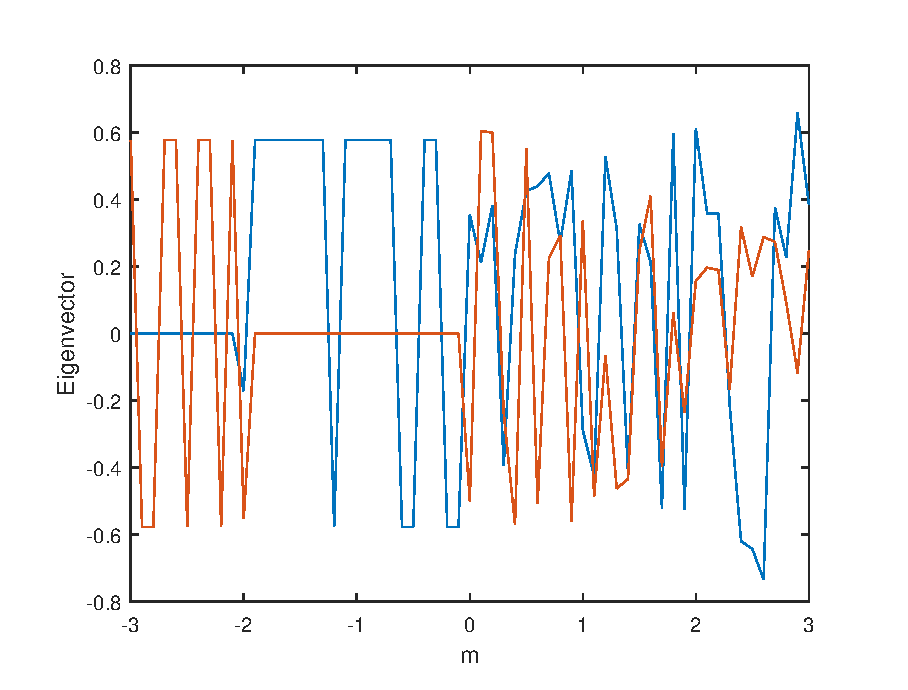
\includegraphics[width=0.6\linewidth]{pics/Eigenvector-m.eps}
\end{figure}

Also, the Mathematica solved eigenvector also demonstrate a
drastical change around $m=-2$. For example, one component, when
plotted against $p_x$ change from:
\begin{figure}[H]
    \centering
    \includegraphics[width=0.6\linewidth]{pics/mN3.pdf}
    \caption{$m=-3$}
\end{figure}
to
\begin{figure}[H]
    \centering
    \includegraphics[width=0.6\linewidth]{pics/{mN2.5}.pdf}
    \caption{$m=-2.5$}
\end{figure}
and suddenly to
\begin{figure}[H]
    \centering
    \includegraphics[width=0.6\linewidth]{pics/mN2.pdf}
    \caption{$m=-2$. There is a discontinuity at $p_x=0$}
\end{figure}
Finaly, it becomes smooth again:
\begin{figure}[H]
    \centering
    \includegraphics[width=0.6\linewidth]{pics/{mN1.5}.pdf}
    \caption{$m=-1.5$}
\end{figure}
The details can be explored in the Mathematica notebook.

Also, the case of $N=4$ is also calculated in Mathematica.
There are similarly two crossing happening at $(m,p_x)$ equals
$(-2,0)$ and $(2,\pm\pi)$.

\begin{figure}[H]
    \centering
    \includegraphics[width=0.6\linewidth]{pics/N8m2.pdf}
    \caption{$m=2$}
\end{figure}
\begin{figure}[H]
    \centering
    \includegraphics[width=0.6\linewidth]{pics/N8m-2.pdf}
    \caption{$m=-2$}
\end{figure}

Surprisingly, the two bands that cross are have exactly the same
function dependence on $p_x$ and $m$ for the cases of $N=3$ and
$N=4$.

\subsection{Why I Think the Lattice Model Hamiltonian is Mildly Wrong}
\label{sec:Why-LatticeM-m-wrong}

I notice that equation (2.19) transformed according to (2.20)
is not exactly equation (2.21), but is:
\begin{align}
    &H =\sum_{p_x,p_y} c^\dagger_{p_x,p_y}\times
    \nonumber\\
    &
    \left[
        2\sin(p_x)\sigma^x + 2\sin(p_y)\sigma^y
        +(2-m-2\cos(p_x)-2\cos(p_y))\sigma^z
    \right] c_{p_x,p_y}
\end{align}
This result does not become the continuum Dirac Hamiltonian as
$p_x,p_y$ goes to zero. Therefore, I suspect that certain
constants should be modified so that:

\begin{align}
    H_{LD} &= \sum_{m,n}\left\{
        \frac{i}{2} \left[ c^\dagger_{m+1,n}\sigma^x c_{m,n}
            - c^\dagger_{m,n}\sigma^x c_{m+1,n}\right]
        + \frac{i}{2} \left[ c^\dagger_{m,n+1}\sigma^y c_{m,n}
            - c^\dagger_{m,n}\sigma^y c_{m,n+1} \right]
        \right.
        \nonumber\\
        &- \frac{1}{2}\left[
            c^\dagger_{m+1,n}\sigma^z c_{m,n}
            + c^\dagger_{m,n}\sigma^z c_{m+1,n}
            + c^\dagger_{m,n+1}\sigma^z c_{m,n}
            + c^\dagger_{m,n}\sigma^z c_{m,n+1}
        \right]
        \nonumber\\
        & \left. + (2-m) c^\dagger_{m,n}\sigma^z c_{m,n}
        \vphantom{\frac12}
    \right\}
\end{align}

This affects the numerical analysis effectively by the replacement
$$\sigma^i \to \frac{1}{2}\sigma^i,\quad
    (2-m) \to 2(2-m) $$

The calculated result is similar to that in the previous section,
except that the band crossing happens at different values of $m$.
\footnote{For example, the eigenvalue of original and the modified equation
(2.21) are plotted in Mathematica notebook "Eq2.21-Demo.nb". Also,
the solution to the infinite cylinder boundary condition has again
two band crossings, each at $(m,p_x)$ equals $(0,0)$ and
$(2,\pm\pi)$ (for $N=3$ case).}
So the essential point is unaltered by the difference in some
constants. However, in the correct calculation, the crossing band
appears at $m=0$, which represents a massless spin-$\frac{1}{2}$
particle. I think this should have some theoretical implications.

\subsection{Solution With Translational Invariance (Bloch States) in
both x and y (Infinite Plane)}

    \subsubsection{Numerical Solution}
    \label{sec:Numerical Solution}


    \textbf{Note 1}: Since the essential point is not altered by the minor
    error in Hamiltonian, as mentioned in
    Section~\ref{sec:Why-LatticeM-m-wrong}. I will continue with the
    Lattice Model Hamiltonian that produce correctly the Dirac Hamiltonian
    in the continuum limit.

    \textbf{Note 2}: Calculation in this part is available in the
    Mathematica notebook "\texttt{Lattice Dirac Model (2+1)-d-2.nb}".

    When the two sides are of open boundary, the problem is quite simple
    and the Fourier-transformed Hamiltonian is (almost) diagonal in
    momentum space. It is (as calculated in \cite{Hughes2009}, eq.2.21):
    \begin{align}
        &H =\sum_{p_x,p_y} c^\dagger_{p_x,p_y}\times
        \nonumber\\
        &
        \left[
            \sin(p_x)\sigma^x + \sin(p_y)\sigma^y
            +(2-m-\cos(p_x)-\cos(p_y))\sigma^z
        \right] c_{p_x,p_y}
    \end{align}

    The eigenvalues of the Hamiltonian of the form
    $\vb{a}\vdot\vb{\sigma}$ are:
    \begin{equation}
        E_1 = \abs{a},\quad E_2 = -\abs{a}
    \end{equation}
    If plotted in $(p_x,p_y)$ plane, we will find several interesting
    crossing happening when $m=0,2,4$:
    \begin{figure}[H]
        \centering
        \includegraphics[width=0.6\linewidth]{pics/OpenBC-inXY/E-m0.pdf}
        \caption{$m=0$}
    \end{figure}
    \begin{figure}[H]
        \centering
        \includegraphics[width=0.6\linewidth]{pics/OpenBC-inXY/E-m2.pdf}
        \caption{$m=2$}
    \end{figure}
    \begin{figure}[H]
        \centering
        \includegraphics[width=0.6\linewidth]{pics/OpenBC-inXY/E-m4.pdf}
        \caption{$m=4$}
    \end{figure}

    The eigenvectors are of the form:
    \begin{equation}
        \begin{pmatrix}
            \phi, \sin(p_x)+i\cos(p_y)
        \end{pmatrix},\quad \begin{pmatrix}
            \psi, \sin(p_x)+i\cos(p_y)
        \end{pmatrix}
    \end{equation}
    where
    \begin{align}
        \phi &=  (2-m-\cos(p_x)-\cos(p_y))+E_1 \\
        \psi &=  (2-m-\cos(p_x)+\cos(p_y))+E_1
    \end{align}
    And besides crossing each other, they have new interesting behavior as
    $m$ varies. When changing from $m=-1$ to $m=6$, they gradually contact
    and exchange the position of each other
    \footnote{You would get more fun if you execute the animation inside
    the Mathematica notebook}:
    \begin{figure}[H]
        \centering
        \includegraphics[width=0.6\linewidth]{pics/OpenBC-inXY/Eigen-mN1.pdf}
        \caption{$m=-1$}
    \end{figure}
    \begin{figure}[H]
        \centering
        \includegraphics[width=0.6\linewidth]{pics/OpenBC-inXY/Eigen-m0.pdf}
        \caption{$m=0$}
    \end{figure}
    \begin{figure}[H]
        \centering
        \includegraphics[width=0.6\linewidth]{pics/OpenBC-inXY/Eigen-m1.pdf}
        \caption{$m=1$}
    \end{figure}
    \begin{figure}[H]
        \centering
        \includegraphics[width=0.6\linewidth]{pics/OpenBC-inXY/Eigen-m2.pdf}
        \caption{$m=2$}
    \end{figure}
    \begin{figure}[H]
        \centering
        \includegraphics[width=0.6\linewidth]{pics/OpenBC-inXY/Eigen-m3.pdf}
        \caption{$m=3$}
    \end{figure}
    \begin{figure}[H]
        \centering
        \includegraphics[width=0.6\linewidth]{pics/OpenBC-inXY/Eigen-m4.pdf}
        \caption{$m=4$}
    \end{figure}
    \begin{figure}[H]
        \centering
        \includegraphics[width=0.6\linewidth]{pics/OpenBC-inXY/Eigen-m6.pdf}
        \caption{$m=6$}
    \end{figure}

\subsection{Solution With Translational Invariance in x, and Open
Boundary in y (Infinite Stripe)}

This amounts to removing the $A$ in top right corner and $C$ in bottom
left corner of eq.\ref{eq:disc-eigeneq}. 
\footnote{The calculation can be found
in file \texttt{Lattice Dirac Model (2+1)-d-4-Infinite Stripe
(N=3).nb}, and file \texttt{Lattice Dirac Model (2+1)-d-4-Infinite
Stripe (N=20).nb}.}
In this case, the crossing bands exists at slightly different value of
$m$, also, there are few sharp transitions from a closed gap state, to an
open gap state. For example, when $N=3$, the band crossing happens at
two range of $m$: from $0.65$ to $1.35$ (shown in
fig~\ref{fig:InfiniteStrip=3-1.jpg}, and from $2.4$ to $3.75$ (shown
in fig~\ref{fig:InfiniteStrip=3-2.jpg}). The cases when $N=10$,
$N=20$, $N=30$ also exhibits similar behavior. They also have almost
two ranges of values for $m$ when two bands close at one point. Their
result are plotted are at fig~\ref{fig:InfiniteStrip=10.jpg},
fig~\ref{fig:InfiniteStrip=20.jpg}, and ... the result for $N=30$ will
be updated here when my program finishes running.

\begin{figure}[htpb]
    \centering
    \includegraphics[width=0.8\linewidth]{pics/InfiniteStrip/{InfiniteStrip.N=3-1}.jpg}
    \caption{Infinite Strip, $N=3$, closes at $p_x=0$}
    \label{fig:InfiniteStrip=3-1.jpg}
\end{figure}
\begin{figure}[htpb]
    \centering
    \includegraphics[width=0.8\linewidth]{pics/InfiniteStrip/{InfiniteStrip.N=3-2}.jpg}
    \caption{Infinite Strip, $N=3$, closes at $p_x=\pi$}
    \label{fig:InfiniteStrip=3-2.jpg}
\end{figure}
\begin{figure}[htpb]
    \centering
    \includegraphics[width=0.8\linewidth]{pics/InfiniteStrip/{InfiniteStrip.N=10}.jpg}
    \caption{Infinite Strip, $N=10$}
    \label{fig:InfiniteStrip=10.jpg}
\end{figure}
\begin{figure}[htpb]
    \centering
    \includegraphics[width=0.8\linewidth]{pics/InfiniteStrip/{InfiniteStrip.N=20}.jpg}
    \caption{Infinite Strip, $N=20$}
    \label{fig:InfiniteStrip=20.jpg}
\end{figure}

As we have seen, the solution by Mathematica is analytically
intractable as $N$ grows larger. Also it would be too time-consuming
if I were to plotting those eigenvectors when $N$ is large. So I
looked for similar things inside the book by Bernevig
\cite{Bernevig2013}, and found the following model.

    \subsubsection{Edge States Analytically Obtained}
    \label{sec:Edge States}
    I will analyse the continuum limit of this model at the point
    $(p_x=0,p_y=0)$, where the energy $E=0$. I also assume that we
    have placed to materials adjacent to each other in $x$ direction.
    I will assume that the two materials are in different topological
    states. For example, if the band cross when $m=0$, then one
    material will have $m<1$, and the other will have $m>0$.
    Therefore, at the interface, we could have $m$ as a function of
    $x$ such that $m(0)=0$.

    This assumption implies that we break translational in both
    direction. So at this point $p_x=0$, $\sin(p_x)\to p_x$ , and is
    replaced by $-i\hbar \partial _x$. Similar for $\sin(p_y)$. So we
    recovered the continuum model:
    \begin{equation}
        H = -i\hbar\partial_x \sigma^x 
        -i\hbar\partial_y \sigma^y -m \sigma^z
    \end{equation}
    The Schrodinger equation is $H\psi =E\psi = 0$ for $E\approx 0$
    around this point. After some calculations, the equation is (with
    $\hbar=1$):
    \begin{equation}
        \left[i\partial_x \sigma^x + i\partial_y \sigma^y +
        m\sigma^z\right] \psi = 0
    \end{equation}
    However, this coupled PDE is hard to solve by Mathematica
    \footnote{See file \texttt{Lattice Dirac Model
    (2+1)-d-3-EdgeStates.nb} for my calculations.}. Therefore, I
    restrict their value on $x$, and solve the ODE:
    \begin{align}
        i\partial_x \psi_2(x) + m\psi_1(x) &= 0 \\
        i\partial_x \psi_1(x) - m\psi_2(x) &= 0
    \end{align}
    If assuming $m(x)$ is in the form of $m(x)=x$, i.e. positive when
    $x>0$, and negative when $x<0$, then the solution is:
    \begin{align}
        \psi_1 (x,y) &= e^{\text{Int}(x)} C(y) \\
        \psi_2 (x,y) &= -i \psi_1(x,y)
    \end{align}
    where $\text{Int}(x)=\int_1^x -m(k)\dd{k}$. $\text{Int}(x)$ has the
    property of goes to $-\infty$ as $x\to \pm\infty$.

    If, on the contrary, assuming $m(x)$ is in the form of $m(x)=-x$, i.e. positive when $x<0$, and negative when $x>0$, then the solution is:
    \begin{align}
        \psi_1 (x,y) &= e^{-\text{Int}(x)} C(y) \\
        \psi_2 (x,y) &= i \psi_1(x,y)
    \end{align}
    In both cases, the function are exponentially decaying wave in the
    interface at $m(0)=0$.

    Paused to think what I have got. I have in essential got a
    solution separated in $x,y$. Therefore, now I re-solve this edge
    mode, using technique of separation of variables 
    \footnote{Actually, I am just mimicking the calculation
    in section 8.8 of \cite{Bernevig2013}.}. 

    Without loss of generality, assume $m(x)$ is like $x$, i.e. it
    goes to $\pm\infty$ as $x\to\pm\infty$. Then, separate the
    wavefunction into:
    \begin{equation}
        \psi(x,y) = \phi_1(x)\phi_2(y)
    \end{equation}
    Assuming we are solving a Schrodinger equation $H\psi=E\psi$, with
    $E$ being very small.  Now, inspired by previous calculation,
    write down directly $\phi_1(x)=e^{-\int_0^x m(x')\dd{x'}}$.  Then,
    the equation decoupled directly into:
    \begin{equation}
        \left(
            -i\sigma_y\partial_y + m(x)\left(i\sigma_x-\sigma_z\right)
        \right)\psi_2(y) = E\psi_2(y)
    \end{equation}
    Since $E$ is small, but $m(x)$ could be very large and is
    independent of $y$, we should make the term $(i\sigma_x-\sigma_z)$
    somehow disappear. This matrix is singular and has only eigenvalue
    $0$. Its eigenvector is $(i,1)^t$. So we assume
    $\phi_2(y)=\chi(x)(i,1)^t$.
    
    It turns out that $(i,1)^t$ is also the eigenvector of
    $\sigma_y$ with eigenvalue $-1$. So the equation becomes quite
    simple now:
    \begin{equation}
        i\partial_y\chi(y) = E\chi(y)
    \end{equation}
    The solution is $\chi(y)=e^{-iEy}$, a free electron in the $y$
    direction!

    \textbf{Remark}: Although I have broken translational symmetry in
    both direction, I could do almost the same calculation with $p_y$
    conserved, e.g. in a infinite strip. In that case, I would get a
    state localized in the interface, and have $p_y=-E$, representing
    an electron travelling with momentum $-E$ in $y$'s direction.
\section{License}
The entire content of this work (including the source code
for TeX files and the generated PDF documents) by 
Hongxiang Chen (nicknamed we.taper, or just Taper) is
licensed under a 
\href{http://creativecommons.org/licenses/by-nc-sa/4.0/}{Creative 
Commons Attribution-NonCommercial-ShareAlike 4.0 International 
License}. Permissions beyond the scope of this 
license may be available at \url{mailto:we.taper[at]gmail[dot]com}.
\bibliography{../../Library}{}
\bibliographystyle{alphaurl}

\printnomenclature

\end{document}
